\documentclass{article}

\usepackage[utf8]{inputenc}

% Figures
\usepackage{graphicx}
\usepackage{float}

% Tables
\usepackage{makecell}
\usepackage{multirow}
\usepackage{rotating}
\usepackage{booktabs}

% BibTeX configuration
\usepackage{biblatex}
\bibliography{references} 
\RequirePackage{doi}
\usepackage{hyperref}




\title{Paths in the labyrinth}
\author{Yannick Lang\\
    \small yannick-stephan.lang@stud.uni-bamberg.de}

\date{ \vspace{0.5cm} \large 
  SME-PHY-B\\ 
  \emph{Physical Computing} \\ \vspace{0.2cm}
  Otto-Friedrich-Universität Bamberg \\ \vspace{0.2cm}
  Summer Term 2022}



\begin{document}

% Custom Commands
\newcommand{\IIC}{I\textsuperscript{2}C}

\maketitle

% Main contents
\section{Introduction}
The following paper describes an arduino based system capable of distinguishing types of junctions via ultrasound.
\section{Setup}
\label{sec:setup}

The following section describes the physical components for the project, 
starting with the actual hardware and also covering the environment.
\subsection{Hardware}
\label{subsec:hardware}

From a hardware perspective, two main platforms are used: an arduino micro controller which captures the output from the sensors and a laptop, which processes the data.

\paragraph{Arduino}
This consists of an arduino Nano v.3, a MPU6050 used for its gyroscope sensor and a ultrasound transducer.

\paragraph{Laptop}
The arduino is connected via mini USB cable to a laptop, which provides the micro controller with power and receives and evaluates sensor data from it.
While this does not need to be a Laptop, for instance a Desktop computer or even a raspberry pi could be used instead, I will refer to this component as a Laptop in the following sections.
\subsection{Environment}
\label{subsec:environment}

For this project, the breadboard, on which the arduino and both sensors are connected, is mounted on a swivel plate.
This allows the for easy and smooth rotation.
The board should be mounted in a way that puts the ultrasound sensor close to its center of rotation.
\section{Software}
\label{sec:software}

The software for this project consists of two main parts: The code for the micro controller, written in C, and the code for the laptop, written in Typescript.
\subsection{Arduino}
\label{subsec:arduino}

As stated previously, the code that controls the arduino is written in C.
Its purpose is to configure the sensors, monitor them for new data and relay that to the Laptop when available.
Communication with the MPU6050 sensor happens via the Inter-Integrated Circuit (\IIC) protocol.
Communication with the laptop uses a serial connection via USB at a BAUD rate of 19200.


The main control logic for the micro controller is quite simple. Upon startup, all ports and sensors are configured.
Then, a infinite loop is started, which relays sensor data to the laptop if a new value is available.
Availability of new sensor data is determined via interrupts.
\subsection{Laptop}
\label{subsec:laptop}

The reasons I choose Typescript for the Laptop-side software are that this is the language I have the most experience with and that, when used in the context of a webapp, it facilitates easy visualization of data.
This is especially helpful for debugging, but comes at the price of performance, which I assume is lower than what can be achieved with other languages such as C.

\paragraph{Proxy}
Because a webapp cannot directly access the serial port, I wrote a proxy script, which reads from the serial port and provides received data via the WebSocket protocol.

\paragraph{Detecting a Rotation}
Detection of a $180\deg$ rotation from left to right is implemented via a state machine.
The relevant sensor values for this detection is the X value of the gyroscope on the MPU6050.
Because the values are not 0 even when the board is completely still, I decided to use the first 50 received values for calibration.
This means that the board should be stable for the first about 2 seconds (see chapter \ref{sec:benchmark}) after connection with the laptop is established.
Those values are used to calculate mean and standard deviation.

If a received value is then within $x$ times the standard deviation of the mean, the platform is considered to not be turning.
If the value is above or below the threshold, the state machine goes to the Over/Under states respectively.
Because outliers are still possible, there are further states, namely Over_Steady and Under_Steady. 
While in the Over/Under states, a counter is maintained, which is increased for each measurement outside the threshold and decreased if the platform is stable again.
If the counter reaches 0, the state returns to the standard, i.e. Steady. If the counter reaches a threshold, 
% TODO: is STEADY above/below really necessary or would Math.max do the trick??? 

% TODO: include visualization of state machine 

\paragraph{Capturing Ultrasound Data}

\paragraph{Normalizing Data}
Due in part to the variable update rate, which is discussed in Section \ref{subsec:benchmark}, the captured readings need to be normalized.
This is done by using the sum of gyroscope readings starting from the beginning of rotation as x-coordinate for the current distance reading.
The total sum of gyroscope readings for a rotation then corresponds to $180\deg$ and other values can be scaled accordingly.

\paragraph{Evaluating Data}
\section{Analysis}
\label{sec:analysis}

\paragraph{Detection of turns}
Detection of turns works very well. The thresholds for detecting a turn from left to right, i.e. a $180\deg$ clockwise turn, have been set to $-170\deg$ and $-210\deg$.
When a the end of a turn is detected, and the sum of the turn translates to a value between those bounds, the turn is deemed to have been valid, i.e. a turn from left to right.
The target of $180\deg$ is not at the center of the interval, because experiments showed it to work more reliable that way.
Reliability in this context refers to the detection rate for turns that feel like they should have been valid.
Because the direction of the turn is regarded as well, measurements can be easily taken and the platform can be rotated back to its initial position without triggering a new measurement (if the platform is turned counter-clockwise in order to go back to the initial position).


\paragraph{Detection of Junctions}
% TODO: this
To help with debugging this, the webapp also includes a section that can generate expected scan data and run the junction detection on this data. This is the same utility that was used to generate the theoretic data before, see \ref{fig:theory}.
The classification with the generated data as input pretty reliably, apart from the corridor scenario, which is sometimes misclassified as X Junction when the corridor width is too small.
\subsection{Benchmarks}
\label{subsec:benchmark}

\paragraph{Frequency of Updates}
To determine the frequency of updates, values received per second where averaged over 100 seconds.
The rate of updates from the gyroscope is very steady, at between 31 and 32 Updates per second.
The frequency of new values from the ultrasound sensor is not as steady, as it depends on the distance being measured.
This is because longer distances take longer to measure, and the arduino immediately starts a new measurement upon completion.
In general, distance measured and update frequency are inversely proportional, i.e. with longer distance the rate of updates decreases.
At 10cm distance, update frequency is about 75Hz, and decreases roughly by about 10hz per meter, see \ref{fig:benchmark}.

\begin{table}
    \centering
    \begin{tabular}{l|lll}
            & Gyroscope & Ultrasound & \\
        \cline{1-3}
        10  & 31.48979  & 74.9898    & \\
        20  & 31.48979  & 73.77319   & \\
        30  & 31.55670  & 72.02040   & \\
        50  & 31.57731  & 73.82653   & \\
        75  & 31.62886  & 72.11224   & \\
        100 & 31.60821  & 65.42857   & \\
        150 & 31.50515  & 55.66326   & \\
        200 & 31.62244  & 53.83673   &
    \end{tabular}

    \caption{Distance in cm from sensor and update frequency}
    \label{table:benchmark}
\end{table}

\begin{figure}
    \centering
    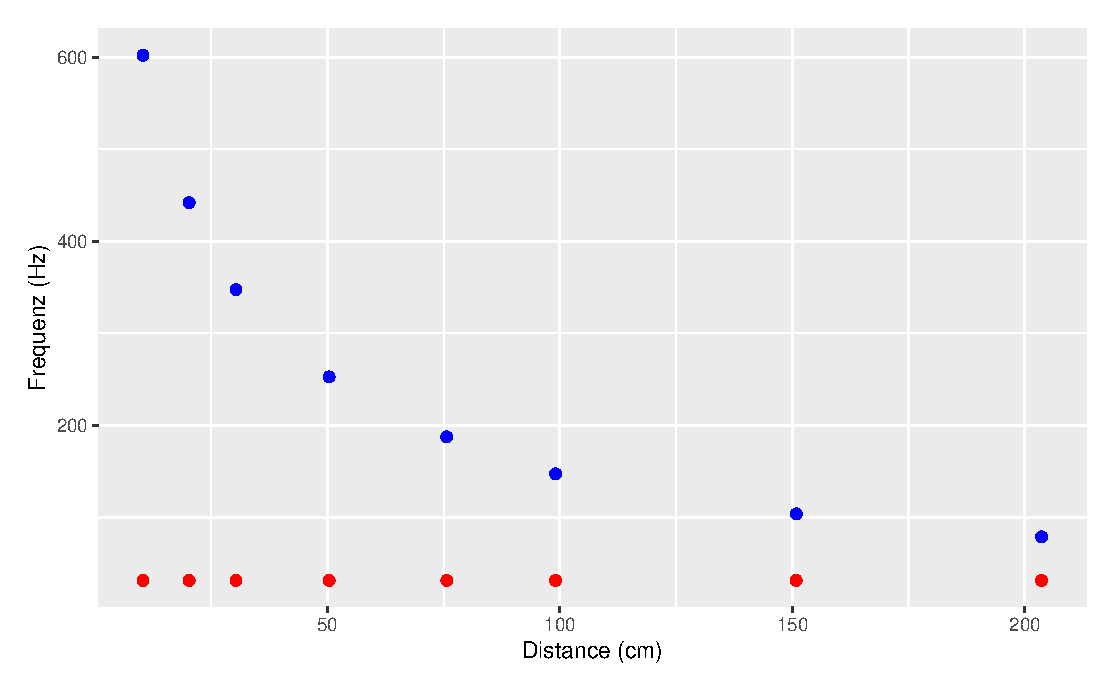
\includegraphics[width=0.5\linewidth]{figures/benchmark.eps}
    \caption{The data from \ref{table:benchmark} visualized}
    \label{fig:benchmark}
\end{figure}


\section{Summary}
\label{sec:summary}

This paper describes the process of building a platform for distinguishing x junctions, t junctions and corridors via a gyroscope and a ultrasonic distance sensor.
Turns of the platform are reliably detected via a state machine.
Upon detection, data that has been recorded during the rotation is used to compare the scan of the environment against previously recorded data, thus allowing a classification.

% Please clean your references! 
% See https://sites.umiacs.umd.edu/elm/2018/12/13/the-art-of-clean-references/
\printbibliography

\end{document}